\begin{frame}{Research Question 1: \\Characteristics from the Planning Problem Representation}
	\begin{itemize}
	\item Use STRIPS to represent the cyber-security and the Rush Hour domains as state transition systems
	\item Define boolean state variables to represent the state (predicates)
	\item Define actions to transition between states using \textbf{preconditions} and \textbf{postconditions}
	\end{itemize}
	
\begin{figure}[!ht]
\noindent\fbox{
 \parbox{\columnwidth}{\raggedright 
{\small
\texttt{\hspace*{5pt}(:action move-car \\
                \hspace*{5pt}:parameters (?v - vehicle ?from ?to ?tail - location \\ \hspace*{40pt}?d - direction)\\
                \hspace*{5pt}:precondition (and (car ?v)(at ?v ?from)\\ \hspace*{40pt}(at ?v ?tail)(face ?v ?d)\\ \hspace*{40pt}(next ?d ?from ?to)(next ?d ?tail ?from)\\ \hspace*{40pt}(free ?to))\\
                \hspace*{5pt}:effect (and (at ?v ?to) (not (at ?v ?tail))(free ?tail)\\\hspace*{35pt}(not (free ?to))))}

}
}
}
\end{figure}

\end{frame}
\begin{frame}{Rush Hour in STRIPS - Initial State}
\begin{figure}[!htb]
  \centering
  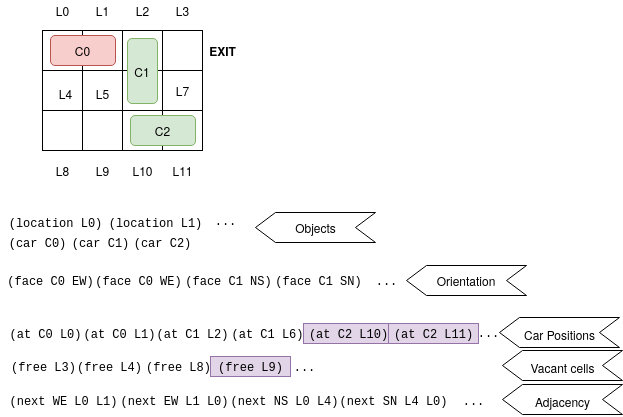
\includegraphics[width=\columnwidth, keepaspectratio=true]{img/s1.png}
\end{figure}
\end{frame}
\begin{frame}{Rush Hour in STRIPS - Next State}
\begin{figure}[!htb]
  \centering
  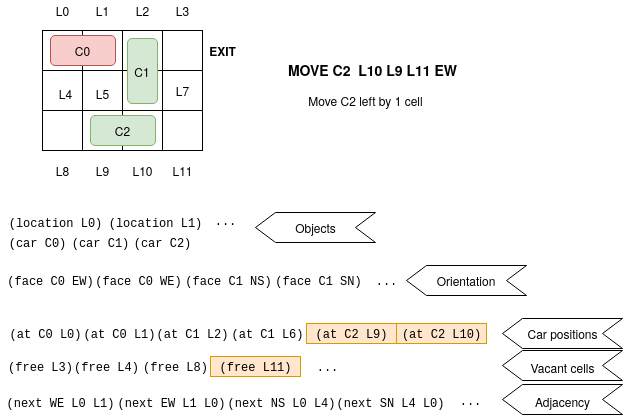
\includegraphics[width=\columnwidth, keepaspectratio=true]{img/s2.png}
\end{figure}
\end{frame}